\documentclass[aspectratio=169]{beamer}

% I sure do use alot of useless packages
%%%%%%%%%%%%%%%%%%%%%%%%%%%%%%%%%%%%%%%%%%%%%%%%%%%%%%%%%%%%%%%%%%%%%%%%%%%%%%
% \embedvideo{<poster or text>}{<video file (MP4+H264)>}
% \embedvideo*{...}{...}                     % auto-play
%%%%%%%%%%%%%%%%%%%%%%%%%%%%%%%%%%%%%%%%%%%%%%%%%%%%%%%%%%%%%%%%%%%%%%%%%%%%%%
\usepackage{xparse}
\usepackage[bigfiles]{pdfbase}
\ExplSyntaxOn
\NewDocumentCommand\embedvideo{smm}{
  \group_begin:
  \leavevmode
  \tl_if_exist:cTF{file_\file_mdfive_hash:n{#3}}{
    \tl_set_eq:Nc\video{file_\file_mdfive_hash:n{#3}}
  }{
    \IfFileExists{#3}{}{\GenericError{}{File~`#3'~not~found}{}{}}
    \pbs_pdfobj:nnn{}{fstream}{{}{#3}}
    \pbs_pdfobj:nnn{}{dict}{
      /Type/Filespec/F~(#3)/UF~(#3)
      /EF~<</F~\pbs_pdflastobj:>>
    }
    \tl_set:Nx\video{\pbs_pdflastobj:}
    \tl_gset_eq:cN{file_\file_mdfive_hash:n{#3}}\video
  }
  %
  \pbs_pdfobj:nnn{}{dict}{
    /Type/RichMediaInstance/Subtype/Video
    /Asset~\video
    /Params~<</FlashVars (
      source=#3&
      skin=SkinOverAllNoFullNoCaption.swf&
      skinAutoHide=true&
      skinBackgroundColor=0x5F5F5F&
      skinBackgroundAlpha=0.75
    )>>
  }
  %
  \pbs_pdfobj:nnn{}{dict}{
    /Type/RichMediaConfiguration/Subtype/Video
    /Instances~[\pbs_pdflastobj:]
  }
  %
  \pbs_pdfobj:nnn{}{dict}{
    /Type/RichMediaContent
    /Assets~<<
      /Names~[(#3)~\video]
    >>
    /Configurations~[\pbs_pdflastobj:]
  }
  \tl_set:Nx\rmcontent{\pbs_pdflastobj:}
  %
  \pbs_pdfobj:nnn{}{dict}{
    /Activation~<<
      /Condition/\IfBooleanTF{#1}{PV}{XA}
      /Presentation~<</Style/Embedded>>
    >>
    /Deactivation~<</Condition/PI>>
  }
  %
  \hbox_set:Nn\l_tmpa_box{#2}
  \tl_set:Nx\l_box_wd_tl{\dim_use:N\box_wd:N\l_tmpa_box}
  \tl_set:Nx\l_box_ht_tl{\dim_use:N\box_ht:N\l_tmpa_box}
  \tl_set:Nx\l_box_dp_tl{\dim_use:N\box_dp:N\l_tmpa_box}
  \pbs_pdfxform:nnnnn{1}{1}{}{}{\l_tmpa_box}
  %
  \pbs_pdfannot:nnnn{\l_box_wd_tl}{\l_box_ht_tl}{\l_box_dp_tl}{
    /Subtype/RichMedia
    /BS~<</W~0/S/S>>
    /Contents~(embedded~video~file:#3)
    /NM~(rma:#3)
    /AP~<</N~\pbs_pdflastxform:>>
    /RichMediaSettings~\pbs_pdflastobj:
    /RichMediaContent~\rmcontent
  }
  \phantom{#2}
  \group_end:
}
\ExplSyntaxOff
%%%%%%%%%%%%%%%%%%%%%%%%%%%%%%%%%%%%%%%%%%%%%%%%%%%%%%%%%%%%%%%%%%%%%%%%%%%%%%

\newcommand{\emptybox}[2][\textwidth]{%
  \begingroup
  \setlength{\fboxsep}{-\fboxrule}%
  \noindent\framebox[#1]{\rule{0pt}{#2}}%
  \endgroup
}

\usepackage[english]{babel}
\usepackage{csquotes}
\usepackage{calc}
\usepackage[absolute,overlay]{textpos}
\usepackage{graphicx}
\usepackage{xcolor}
\usepackage{subfig}
\usepackage{multimedia}
\usepackage{amsmath}
\usepackage{amsfonts}
% \usepackage{amsthm}
\usepackage{mathtools}
\usepackage{comment}
% \usepackage{MnSymbol,wasysym}
% \usepackage{textcomp}
\usepackage{hyperref}
\usepackage{multimedia}
\usepackage[]{booktabs} % For \toprule, \midrule and \bottomrule
\usepackage[round-mode=places, round-integer-to-decimal, round-precision=2,
    table-format = 1.2, 
    table-number-alignment=center,
    round-integer-to-decimal,
    output-decimal-marker={.}
    ]{siunitx}

% Niels custom packages!
\usepackage{nielstikz}
\usepackage[]{tikz-3dplot}
\usepackage[]{pgfplots}
\usepackage{blox}
\usetikzlibrary{arrows}
\usetikzlibrary{circuits}

\pgfplotsset{compat=1.16}
\pgfplotsset{scaled x ticks=false}
\usetikzlibrary{pgfplots.groupplots}
\usetikzlibrary{pgfplots.fillbetween}
\usetikzlibrary{patterns}
\usetikzlibrary{external}

% Assumes linux 
\immediate\write18{mkdir build/tikz-output}
\makeatletter
\tikzset{external/shell escape={-shell-escape\space-output-directory=build}}
\makeatother
% \tikzexternalize[prefix=tikz-output/]

\usepackage{nielstex}

\newcommand\hmmax{0}
\newcommand\bmmax{0}

% =Definitions===========================================================================
% Thesis specific definitions
\newcommand{\za}{\mathrm{A}}
\newcommand{\zb}{\mathrm{B}}
\newcommand{\zz}{\mathcal{Z}}

% Set theme
\setbeamertemplate{navigation symbols}{} % remove navigation symbols
\mode<presentation>{\usetheme{tud}}

% Bibliography settings 
\usepackage[backend=bibtex,giveninits=true,maxnames=30,maxcitenames=20,url=false,style=authoryear]{biblatex}
\bibliography{bibliography}
\setlength\bibitemsep{0.3cm} % space between entries in the reference list
\renewcommand{\bibfont}{\normalfont\scriptsize}
\setbeamerfont{footnote}{size=\tiny}
\renewcommand{\cite}[1]{\footnote<.->[frame]{\fullcite{#1}}}
\newcommand{\te}[1]{\vspace{10pt}\textbf{Time Estimate: #1}}

% Front page settings
\title{\textbf{Sound Zones with a Cost Function based on Human Hearing}}
% \subtitle{test}
\institute[]{Delft University of Technology, The Netherlands\\
Bang and Olufsen, Denmark}
\author{Niels de Koeijer\\{ MSc Thesis Defence}}
\date{September 16, 2021}

\begin{document}

% Introduction Slide
{\setbeamertemplate{footline}{\usebeamertemplate*{minimal footline}} \frame{\titlepage}}

\note{
    Welcome to my MSc thesis defence.\\
    The title of my MSc thesis is:\\
            \begin{center}
            ``Sound Zones with a Cost Function based on Human Hearing''.
            \end{center}
    And I would like to tell you all about it.\\
    \te{00:20}
}

% Part I: introduction to the project
\begin{frame}{\textbf{Preface:} About Me}
    % Who I am, what, why
    \begin{columns}[c]
        \column{.60\textwidth}
        \begin{block}{\textbf{Niels de Koeijer}}
        Master Student at:
        \begin{itemize}
            \item Delft University of Technology,
            \item Research Department at Bang \& Olufsen.
        \end{itemize} 
        \end{block}
        \column{.33\textwidth}
        \begin{figure}
            \vspace{-0.8cm}
            \centering
            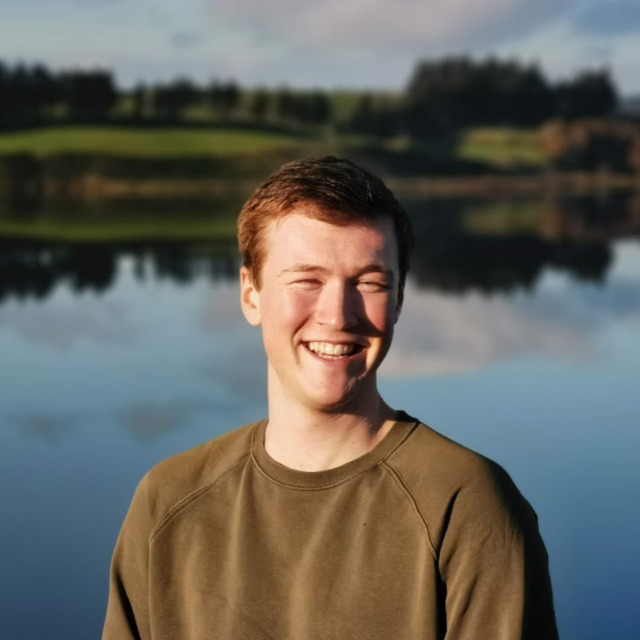
\includegraphics[scale=0.17]{me.jpg}
        \end{figure}
    \end{columns}
\end{frame}

\note{
    First, a little about me: I am Niels.\\
    Aside from the signals and systems group here at TU Delft, I did my MSc thesis in part at a company.\\
    Namely the audio compnay Bang and Olufsen located in Denmark.\\
    \te{00:20}
}

\begin{frame}{\textbf{Preface:} The Sound Zone Problem I}
    \begin{center}
        ``Using an \textbf{array~of~loudspeakers} to create \textbf{zones~of~distinct~audio} with \textbf{minimal~interference} in a room.''
    \end{center}
    \begin{figure}[]
        \centering
        \scalebox{0.7}{\begin{tikzpicture}
    \tikzset{
      Speaker/.pic={
        \filldraw[fill=gray!40,pic actions] 
        (-15pt,0) -- 
          coordinate[midway] (-front) 
        (15pt,0) -- 
        ++([shift={(-6pt,8pt)}]0pt,0pt) coordinate (aux1) -- 
        ++(-18pt,0) coordinate (aux2) 
        -- cycle 
        (aux1) -- ++(0,6pt) -- coordinate[midway] (-back) ++(-18pt,0) -- (aux2);
      }
    }

    \draw [draw=black] (0,0) rectangle (8,6);

    % Speakers on the top wall
    \pic[scale=0.7] at (2, 5.6) {Speaker};
    \pic[scale=0.7] at (3, 5.6) {Speaker};
    \pic[scale=0.7] at (4, 5.6) {Speaker};
    \pic[scale=0.7] at (5, 5.6) {Speaker};
    \pic[scale=0.7] at (6, 5.6) {Speaker};

    % Speakers on the bottom wall
    \pic[rotate=180, scale=0.7] at (2, 0.4) {Speaker};
    \pic[rotate=180, scale=0.7] at (3, 0.4) {Speaker};
    \pic[rotate=180, scale=0.7] at (4, 0.4) {Speaker};
    \pic[rotate=180, scale=0.7] at (5, 0.4) {Speaker};
    \pic[rotate=180, scale=0.7] at (6, 0.4) {Speaker};

    \draw[opacity=0.4, fill=blue] (6,3) circle[radius=1.5];
    \draw[thick] (6,3) circle (1.5) node[align=center] {\textbf{Zone B:}\\Music};
    \draw[opacity=0.4, fill=red]  (2,3) circle[radius=1.5];
    \draw[thick] (2,3) circle (1.5) node[align=center] {\textbf{Zone A:}\\Movie};
\end{tikzpicture}
}
    \end{figure}
\end{frame}

\note{
    During my MSc I worked on something called sound zones.\\
    In sound zones the idea is essentially to:\\
    \begin{center}
        ``Use an \textbf{array~of~loudspeakers} to create \textbf{zones~of~distinct~audio} with \textbf{minimal~interference} in a room.''
    \end{center}
    So, in this image, we have a room with two zones.\\
    In one zone we want to reproduce the audio of a movie, and in the other zone we want to reproduce music.\\
    A sound zone algorithm calculates how an array of loudspeakers can be used to reproduce both zones with minimal interference.\\
    So when I am standing here in zone B I only hear music: I do not hear the movie.\\
    This way, multiple people in the same room can enjoy separate audio content without bothering one another.

    \te{00:20}
}

\begin{frame}{\textbf{Preface:} The Sound Zone Problem II}
    \centering
    \embedvideo{\emptybox[8cm]{5cm}}{./intro-animation.mp4}
\end{frame}

\note{
    Of course, it is much easier if I show you an example.\\
    Here I have created two zones with different content, and I will show you what you hear in each zone.\\
    As you can hear, you hear the content of one zone, and then we fly to the other, and it slowly changes to the content of the other zone.\\
    I can play it again.
}

\begin{frame}{\textbf{Preface:} Introducing Perceptual Sound Zones}
    \begin{columns}[c]
        \column{.60\textwidth}
        \begin{block}{\textbf{Thesis Approach}}
            \begin{itemize}
                \item \textbf{Goal of Thesis:}\\ Include a model of the human auditory system in sound zone algorithms.
                \item \textbf{Motivation:}\\ Optimize what matters to humans perceptually.
            \end{itemize}
        \end{block}
        \column{.33\textwidth}
        \begin{figure}
            \centering
            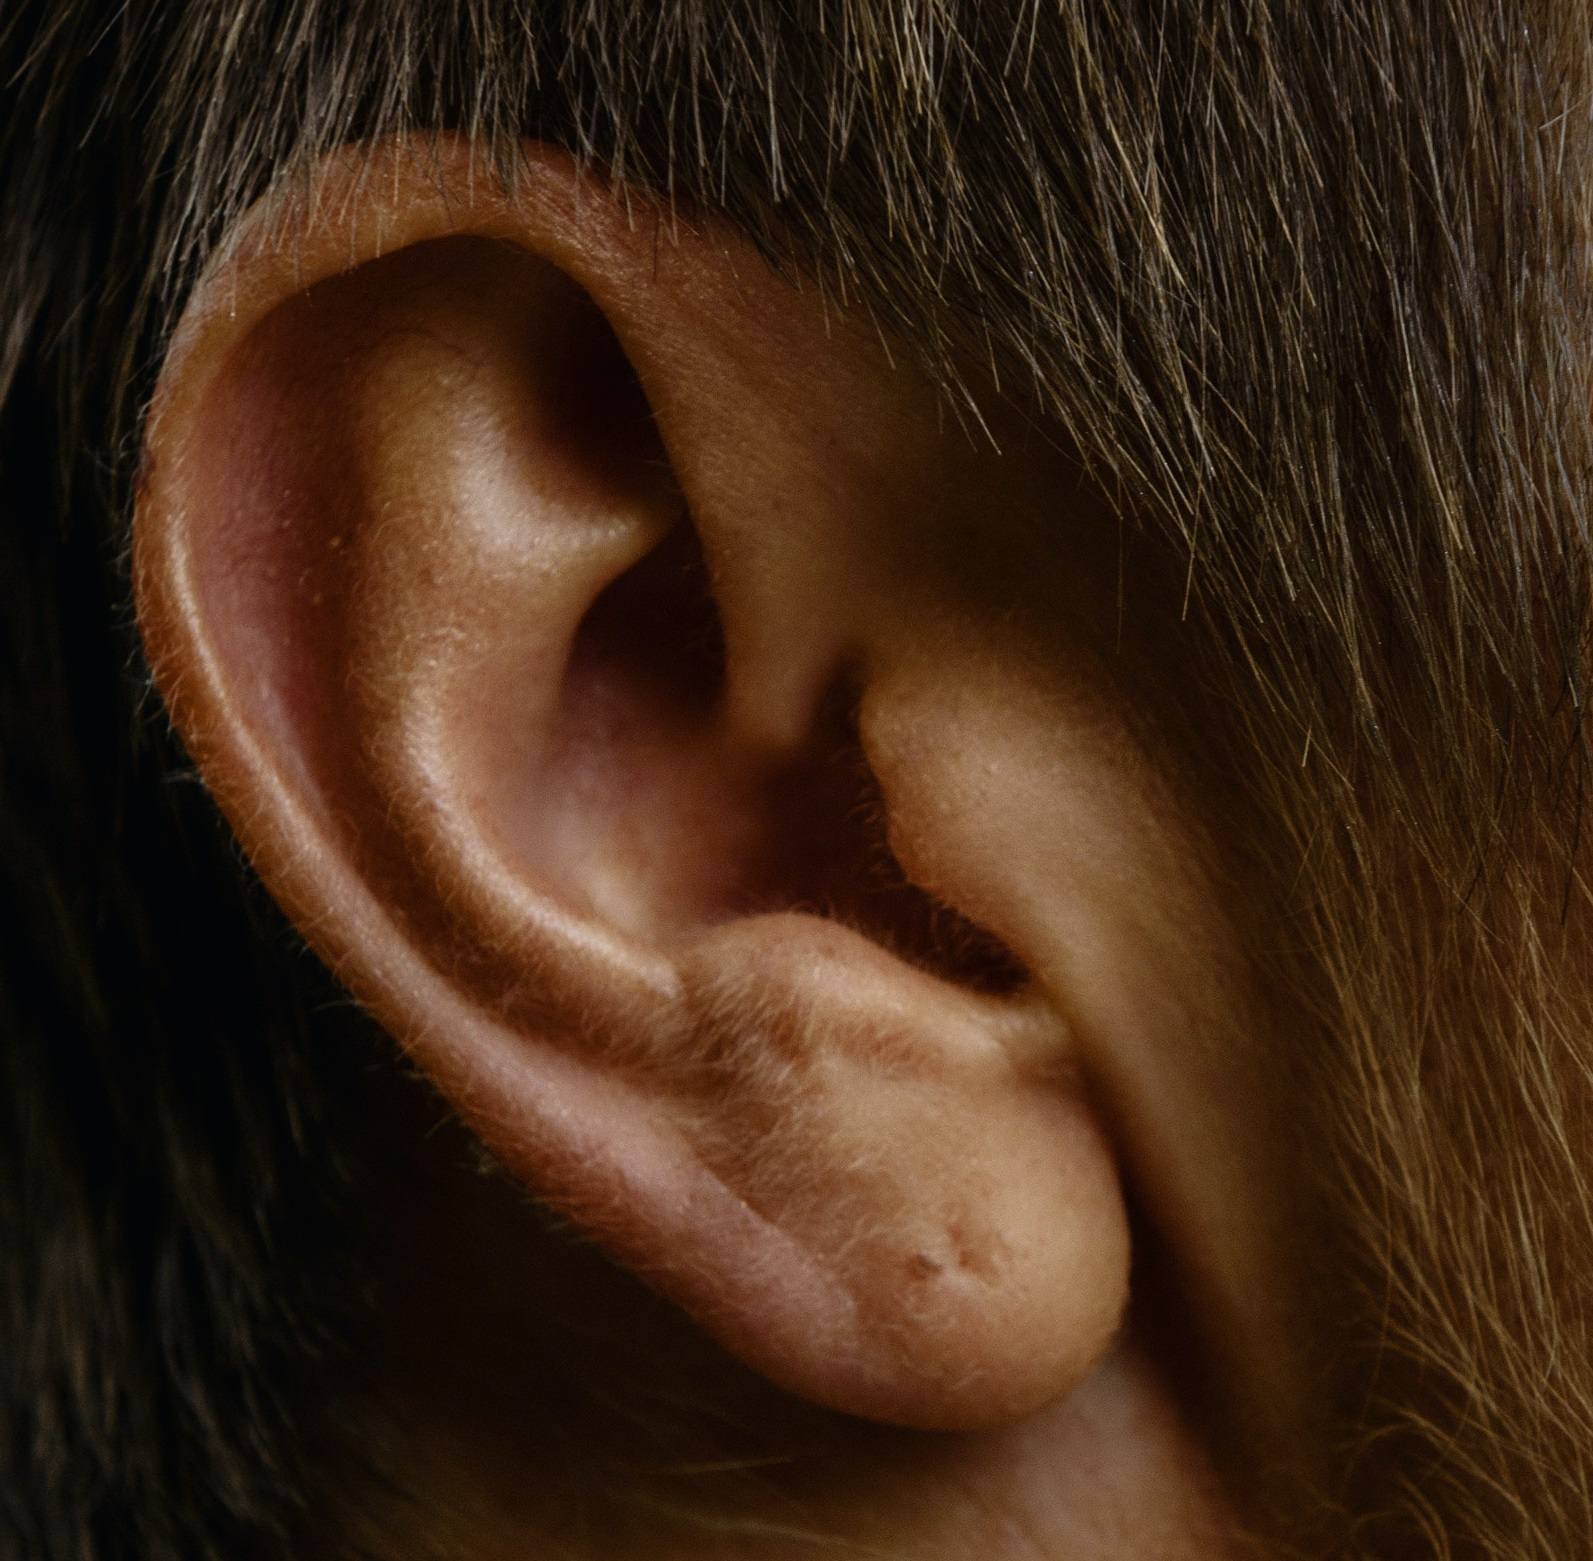
\includegraphics[scale=0.07]{ear.jpg}
        \end{figure}
    \end{columns}
\end{frame}

\note{
    So, now for what I tried to do in my thesis.\\
    In my thesis, I sought to improve sound zones by including a model of the human auditory system into sound zone algorithms.\\
    A model of the human auditory system models how humans perceive sound.\\
    Usually, sound zone algorithms optimize the sound pressure in the room to match what we want.\\
    Sound pressure is a very physical quantity.\\
    This quantity usually does not correspond well with how humans actually perceive sound.\\
    It doesn't take into account what the human ear is sensitive for.\\
    As such, optimizing over a perceptual model instead allows us to optimize over what matters perceptually to humans.
}

\begin{frame}{\textbf{Preface:} Research Questions}
    \begin{block}{\textbf{RQ1:}}
        \begin{center}
            \vspace{\baselineskip}
            \textbf{``How can perceptual models be included in sound~zone~algorithms?''}\\\vspace{\baselineskip}
        \end{center}
    \end{block}
    \begin{block}{\textbf{RQ2:}}
        \begin{center}
            \vspace{\baselineskip}
            \textbf{``What are benefits of including perceptual models in sound zone algorithms?''}\\\vspace{\baselineskip}
        \end{center}
    \end{block}
\end{frame}

\note{
    To guide my investigation into including perceptual information in sound zone algorithms, I posed two research questions.\\
    The first research question is:
    \begin{center}
        \textbf{``How can perceptual models be included in sound~zone~algorithms?''}
    \end{center}
    So, how do we create these perceptual sound zone algorithms.\\
    The second research question is:
    \begin{center}
        \textbf{``What are benefits of including perceptual models in sound zone algorithms?''}
    \end{center}
    So, when we have created these perceptual sound zone algorithms, what are the benefits?
}

% [WIP] Structure slide
\begin{frame}{\textbf{Structure:} Answering Research Question 1}
    \begin{block}{\textbf{RQ1:} How can perceptual models be included in sound~zone~algorithms?}
        \begin{enumerate}
            \item \textbf{Finding a suitable perceptual model}
                \\\phantom{{$\mathbf{\checkmark}$} The Par distortion detectability perceptual model}
                \vspace{3pt}
            \item \textbf{Proposal of a perceptual sound zone framework}
                \\\phantom{{$\mathbf{\checkmark}$} Framework of the detectability of sound pressure errors from pressure matching}
                \vspace{3pt}
            \item \textbf{Proposal of perceptual sound zone algorithms}
                \\\phantom{{$\mathbf{\checkmark}$} Proposal of unconstrained and constrained perceptual pressure matching}
                \vspace{3pt}
        \end{enumerate}
    \end{block}
\end{frame}
\note{
    We will start by answering the first research question.\\
    This will be done in three steps.\\
    In the first step, we will seek to find a perceptual model for use in our perceptual sound zone algorithm.\\
    Then, in the next step, we will propose a perceptual sound zone framework which uses the perceptual model.\\
    This perceptual sound zone framework will then be used in the third step to propose perceptual sound zone algorithms.
}
\begin{frame}{\textbf{Structure:} Answering Research Question 1}
    \begin{block}{\textbf{RQ1:} How can perceptual models be included in sound~zone~algorithms?}
        \begin{enumerate}
            \item \underline{\textbf{Finding a suitable perceptual model}}
                \\\phantom{{$\mathbf{\checkmark}$} The Par distortion detectability perceptual model}
                \vspace{3pt}
            \item \textbf{Proposal of a perceptual sound zone framework}
                \\\phantom{{$\mathbf{\checkmark}$} Framework of the detectability of sound pressure errors from pressure matching}
                \vspace{3pt}
            \item \textbf{Proposal of perceptual sound zone algorithms}
                \\\phantom{{$\mathbf{\checkmark}$} Proposal of unconstrained and constrained perceptual pressure matching}
                \vspace{3pt}
        \end{enumerate}
    \end{block}
\end{frame}
\note{
    We will start now with the first step: finding a suitable perceptual model.
}

\begin{frame}{\textbf{Finding a Perceptual Model:} Par Distortion Detectability Introduction}
    A perceptual model is found through literature review:
    \begin{block}
        {\textbf{Par distortion detectability}\cite{van2005perceptual}} 
        \begin{itemize}
            \item Defines a mathematical function $D(x[n], \varepsilon[n])$.
            \vspace{3pt}
            \item Quantifies how easily a \textbf{human~listener} can \textbf{detect~disturbance} audio $\varepsilon[n]$ when \textbf{also~listening~to} masking audio $x[n]$.
            \vspace{3pt}
            \item It is used in \textbf{audio coding} to hide compression artifacts. 
            \vspace{3pt}
        \end{itemize}
    \end{block}
\end{frame}

\begin{frame}{\textbf{Finding a Perceptual Model:} Par Distortion Detectability Workings}
    % The Par distortion detectability determines how detectable disturbance $\varepsilon[n]$ is through: 
    \begin{block}
        {\textbf{Psycho-Acoustical Principals}}
        \begin{itemize}
            \item \textbf{Threshold of Hearing:}\\The lowest sound pressure level humans can hear.
            \vspace{3pt}
            \item \textbf{Auditory Masking:}\\
                The degree to which $x[n]$ ``overpowers'' disturbance $\varepsilon[n]$.  
            \vspace{3pt}
        \end{itemize}
    \end{block}
\end{frame}

\begin{frame}{\textbf{Structure:} Answering Research Question 1}
    \begin{block}{\textbf{RQ1:} How can perceptual models be included in sound~zone~algorithms?}
        \begin{enumerate}
            \item \textbf{Finding a suitable perceptual model}
                \\{{$\mathbf{\checkmark}$} The Par distortion detectability perceptual model}\vspace{3pt}
            \item \textbf{Proposal of a perceptual sound zone framework}
                \\\phantom{{$\mathbf{\checkmark}$} Framework of the detectability of sound pressure errors from pressure matching}\vspace{3pt}
            \item \textbf{Proposal of perceptual sound zone algorithms}
                \\\phantom{{$\mathbf{\checkmark}$} Proposal of unconstrained and constrained perceptual pressure matching}\vspace{3pt}
        \end{enumerate}
    \end{block}
\end{frame}

\begin{frame}{\textbf{Structure:} Answering Research Question 1}
    \begin{block}{\textbf{RQ1:} How can perceptual models be included in sound~zone~algorithms?}
        \begin{enumerate}
            \item \textbf{Finding a suitable perceptual model}
                \\{{$\mathbf{\checkmark}$} The Par distortion detectability perceptual model}\vspace{3pt}
            \item \underline{\textbf{Proposal of a perceptual sound zone framework}}
                \\\phantom{{$\mathbf{\checkmark}$} Framework of the detectability of sound pressure errors from pressure matching}\vspace{3pt}
            \item \textbf{Proposal of perceptual sound zone algorithms}
                \\\phantom{{$\mathbf{\checkmark}$} Proposal of unconstrained and constrained perceptual pressure matching}\vspace{3pt}
        \end{enumerate}
    \end{block}
\end{frame}

\begin{frame}{\textbf{Perceptual Sound Zone Framework:} Pressure Matching I}
    A sound zone approach suitable for integration with the Par distortion detectability is found through literature review:
    \begin{block}
        {\textbf{Pressure Matching Sound Zone Algorithm}\cite{betlehem2015personal}} 
        \begin{itemize}
            \item Controls the sound pressure at \textbf{discrete points} in the room.
            \vspace{3pt}
            \item Minimizes \textbf{``sound pressure errors''} to create sound zones.
            \vspace{3pt}
        \end{itemize}
    \end{block}
\end{frame}

\begin{frame}{\textbf{Perceptual Sound Zone Framework:} Pressure Matching II}
    \begin{center}
        The zones are sampled into $M$ \textbf{``control points''} where we attempt to control the sound by \textbf{controlling~the~inputs} to the $L$ \textbf{loudspeakers} in the room.
    \end{center}
    \begin{columns}[c]
        \centering
        \column{.33\textwidth}
        \begin{figure}[]
            \centering
            \scalebox{0.6}{\begin{tikzpicture} 
    \draw [draw=black] (0,0) rectangle (8,6);

    % Speakers on the top wall
    \pic[scale=0.7] at (2.5, 5.6) {Speaker};
    \pic[scale=0.7] at (3.5, 5.6) {Speaker};
    \pic[scale=0.7] at (4.5, 5.6) {Speaker};
    \pic[scale=0.7] at (5.5, 5.6) {Speaker};

    % Speakers on the bottom wall
    \pic[rotate=180, scale=0.7] at (2.5, 0.4) {Speaker};
    \pic[rotate=180, scale=0.7] at (3.5, 0.4) {Speaker};
    \pic[rotate=180, scale=0.7] at (4.5, 0.4) {Speaker};
    \pic[rotate=180, scale=0.7] at (5.5, 0.4) {Speaker};

    \draw[opacity=0.4, fill=blue] (6,3) circle[radius=1.5];
    \draw[thick] (6,3) circle (1.5) node[align=center] {\textbf{Zone $\text{B}$}};
    \draw[opacity=0.4, fill=red]  (2,3) circle[radius=1.5];
    \draw[thick] (2,3) circle (1.5) node[align=center] {\textbf{Zone $\text{A}$}};
\end{tikzpicture}
}
        \end{figure}
        \column{.10\textwidth}
        \begin{center}
            \Huge$\rightarrow$
        \end{center}
        \column{.33\textwidth}
        \begin{figure}[]
            \centering
            \scalebox{0.6}{\begin{tikzpicture} 
    \draw [draw=black] (0,0) rectangle (8,6);

    % Speakers on the top wall
    \pic[scale=0.7] at (2.5, 5.6) {Speaker};
    \pic[scale=0.7] at (3.5, 5.6) {Speaker};
    \pic[scale=0.7] at (4.5, 5.6) {Speaker};
    \pic[scale=0.7] at (5.5, 5.6) {Speaker};

    % Speakers on the bottom wall
    \pic[rotate=180, scale=0.7] at (2.5, 0.4) {Speaker};
    \pic[rotate=180, scale=0.7] at (3.5, 0.4) {Speaker};
    \pic[rotate=180, scale=0.7] at (4.5, 0.4) {Speaker};
    \pic[rotate=180, scale=0.7] at (5.5, 0.4) {Speaker};

    \draw[opacity=0.7, pattern=wide2] (6,3) circle[radius=1.5];
    \draw[opacity=0.4, fill=blue] (6,3) circle[radius=1.5];
    \draw[thick] (6,3) circle (1.5) node[align=center] {\textbf{Zone $\text{B}$}};
    \draw[opacity=0.7, pattern=wide2]  (2,3) circle[radius=1.5];
    \draw[opacity=0.4, fill=red]  (2,3) circle[radius=1.5];
    \draw[thick] (2,3) circle (1.5) node[align=center] {\textbf{Zone $\text{A}$}};
\end{tikzpicture}
}
        \end{figure}
    \end{columns}
\end{frame}

\begin{frame}{\textbf{Perceptual Sound Zone Framework:} Pressure Matching III}
    \begin{columns}[c]
        \centering
        \column{.60\textwidth}
        \begin{block}{\textbf{Pressure Matching Quantities}}
            For each loudspeaker $l$:
            \begin{itemize}
                \item \textbf{Input signal} $x_A^{(l)}[n]$ and $x_B^{(l)}[n]$.
                \vspace{3pt}
            \end{itemize}
            \vspace{3pt}
            For each point $m$: 
            \begin{itemize}
                \item \textbf{Target sound pressure} $t_A^{(m)}[n]$ and $t_B^{(m)}[n]$. 
                \vspace{3pt}
                \item \textbf{Resulting sound pressure} $p_A^{(m)}[n]$ and $p_B^{(m)}[n]$.
                \vspace{3pt}
            \end{itemize}
        \end{block}
        % \begin{block}{\textbf{Relationship Input and Resulting Sound}}
        %     \begin{itemize}
        %         \item Through \textbf{room impulse responses} $h^{(l,m)}[n]$:
        %            \begin{equation}
        %                p_A^{(m)}[n] = \sum_l \left(h^{(l,m)} \ast x_A^{(l)}\right)[n]
        %            \end{equation} 
        %     \end{itemize}
        % \end{block}
        \column{.33\textwidth}
        \topskip0pt
        \vspace*{\fill}
        \begin{figure}[]
            \centering
            \scalebox{0.6}{\begin{tikzpicture} 
    \draw [draw=black] (0,0) rectangle (8,6);

    % Speakers on the top wall
    \pic[scale=0.7] at (2.5, 5.6) {Speaker};
    \pic[scale=0.7] at (3.5, 5.6) {Speaker};
    \pic[scale=0.7] at (4.5, 5.6) {Speaker};
    \pic[scale=0.7] at (5.5, 5.6) {Speaker};

    % Speakers on the bottom wall
    \pic[rotate=180, scale=0.7] at (2.5, 0.4) {Speaker};
    \pic[rotate=180, scale=0.7] at (3.5, 0.4) {Speaker};
    \pic[rotate=180, scale=0.7] at (4.5, 0.4) {Speaker};
    \pic[rotate=180, scale=0.7] at (5.5, 0.4) {Speaker};

    \draw[opacity=0.7, pattern=wide2] (6,3) circle[radius=1.5];
    \draw[opacity=0.4, fill=blue] (6,3) circle[radius=1.5];
    \draw[thick] (6,3) circle (1.5) node[align=center] {\textbf{Zone $\text{B}$}};
    \draw[opacity=0.7, pattern=wide2]  (2,3) circle[radius=1.5];
    \draw[opacity=0.4, fill=red]  (2,3) circle[radius=1.5];
    \draw[thick] (2,3) circle (1.5) node[align=center] {\textbf{Zone $\text{A}$}};
\end{tikzpicture}
}
        \end{figure}
        \vspace*{\fill}
    \end{columns}
\end{frame}

% \begin{frame}{\textbf{Perceptual Sound Zone Framework:} Pressure Matching IV}
%     \begin{columns}[c]
%         \centering
%         \column{.60\textwidth}
%         \begin{block}{\textbf{Pressure Matching Errors}}
%             \begin{itemize}
%                 \item \textbf{Reproduction error:} 
%                     \begin{align}
%                         \text{RE}^{(m)} &= 
%                             \begin{cases}
%                                 \norm[2][2]{t_A^{(m)} - p_A^{(m)}} & \forall\,m\in\,\text{Zone A} \\[10pt]
%                                 \norm[2][2]{t_B^{(m)} - p_B^{(m)}} & \forall\,m\in\,\text{Zone B}
%                             \end{cases}\\
%                             \intertext{\item \textbf{Leakage error:}}
%                                 \text{LE}^{(m)} &= 
%                             \begin{cases}
%                                 \norm[2][2]{p_B^{(m)}} & \forall\,m\in\,\text{Zone A} \\[10pt]
%                                 \norm[2][2]{p_A^{(m)}} & \forall\,m\in\,\text{Zone B}
%                             \end{cases}
%                     \end{align}
%             \end{itemize}
%         \end{block}
%         \column{.33\textwidth}
%         \topskip0pt
%         \vspace*{\fill}
%         \begin{figure}[]
%             \centering
%             \scalebox{0.6}{\begin{tikzpicture} 
    \draw [draw=black] (0,0) rectangle (8,6);

    % Speakers on the top wall
    \pic[scale=0.7] at (2.5, 5.6) {Speaker};
    \pic[scale=0.7] at (3.5, 5.6) {Speaker};
    \pic[scale=0.7] at (4.5, 5.6) {Speaker};
    \pic[scale=0.7] at (5.5, 5.6) {Speaker};

    % Speakers on the bottom wall
    \pic[rotate=180, scale=0.7] at (2.5, 0.4) {Speaker};
    \pic[rotate=180, scale=0.7] at (3.5, 0.4) {Speaker};
    \pic[rotate=180, scale=0.7] at (4.5, 0.4) {Speaker};
    \pic[rotate=180, scale=0.7] at (5.5, 0.4) {Speaker};

    \draw[opacity=0.7, pattern=wide2] (6,3) circle[radius=1.5];
    \draw[opacity=0.4, fill=blue] (6,3) circle[radius=1.5];
    \draw[thick] (6,3) circle (1.5) node[align=center] {\textbf{Zone $\text{B}$}};
    \draw[opacity=0.7, pattern=wide2]  (2,3) circle[radius=1.5];
    \draw[opacity=0.4, fill=red]  (2,3) circle[radius=1.5];
    \draw[thick] (2,3) circle (1.5) node[align=center] {\textbf{Zone $\text{A}$}};
\end{tikzpicture}
}
%         \end{figure}
%         \vspace*{\fill}
%     \end{columns}
% \end{frame}

\begin{frame}{\textbf{Perceptual Sound Zone Framework:} Pressure Matching IV}
    \begin{columns}[c]
        \centering
        \column{.60\textwidth}
        \begin{block}{\textbf{Pressure Matching Errors}}
            \begin{itemize}
                \item \textbf{Reproduction error for point $m$ in zone A:} 
                    \begin{align}
                        \text{RE}^{(m)} &= 
                                \norm[2][2]{t_A^{(m)} - p_A^{(m)}} 
                \intertext{\item \textbf{Leakage error for point $m$ in zone A:}}
                        \text{LE}^{(m)} &= 
                                \norm[2][2]{p_B^{(m)}} 
                    \end{align}
            \end{itemize}
        \end{block}
        \column{.33\textwidth}
        \topskip0pt
        \vspace*{\fill}
        \begin{figure}[]
            \centering
            \scalebox{0.6}{\begin{tikzpicture} 
    \draw [draw=black] (0,0) rectangle (8,6);

    % Speakers on the top wall
    \pic[scale=0.7] at (2.5, 5.6) {Speaker};
    \pic[scale=0.7] at (3.5, 5.6) {Speaker};
    \pic[scale=0.7] at (4.5, 5.6) {Speaker};
    \pic[scale=0.7] at (5.5, 5.6) {Speaker};

    % Speakers on the bottom wall
    \pic[rotate=180, scale=0.7] at (2.5, 0.4) {Speaker};
    \pic[rotate=180, scale=0.7] at (3.5, 0.4) {Speaker};
    \pic[rotate=180, scale=0.7] at (4.5, 0.4) {Speaker};
    \pic[rotate=180, scale=0.7] at (5.5, 0.4) {Speaker};

    \draw[opacity=0.7, pattern=wide2] (6,3) circle[radius=1.5];
    \draw[opacity=0.4, fill=blue] (6,3) circle[radius=1.5];
    \draw[thick] (6,3) circle (1.5) node[align=center] {\textbf{Zone $\text{B}$}};
    \draw[opacity=0.7, pattern=wide2]  (2,3) circle[radius=1.5];
    \draw[opacity=0.4, fill=red]  (2,3) circle[radius=1.5];
    \draw[thick] (2,3) circle (1.5) node[align=center] {\textbf{Zone $\text{A}$}};
\end{tikzpicture}
}
        \end{figure}
        \vspace*{\fill}
    \end{columns}
\end{frame}

\begin{frame}{\textbf{Perceptual Sound Zone Framework:} Pressure Matching V}
    \begin{columns}[c]
        \centering
        \column{.60\textwidth}
        \begin{block}{\textbf{Pressure Matching}}
            Minimize the sum of reproduction and leakage errors:
            \begin{equation}
                \argmin{x_A^{(l)},\,x_B^{(l)}}{\sum_m \text{RE}^{(m)} + \text{LE}^{(m)}}
            \end{equation}
        \end{block}
        \column{.33\textwidth}
        \topskip0pt
        \vspace*{\fill}
        \begin{figure}[]
            \centering
            \scalebox{0.6}{\begin{tikzpicture} 
    \draw [draw=black] (0,0) rectangle (8,6);

    % Speakers on the top wall
    \pic[scale=0.7] at (2.5, 5.6) {Speaker};
    \pic[scale=0.7] at (3.5, 5.6) {Speaker};
    \pic[scale=0.7] at (4.5, 5.6) {Speaker};
    \pic[scale=0.7] at (5.5, 5.6) {Speaker};

    % Speakers on the bottom wall
    \pic[rotate=180, scale=0.7] at (2.5, 0.4) {Speaker};
    \pic[rotate=180, scale=0.7] at (3.5, 0.4) {Speaker};
    \pic[rotate=180, scale=0.7] at (4.5, 0.4) {Speaker};
    \pic[rotate=180, scale=0.7] at (5.5, 0.4) {Speaker};

    \draw[opacity=0.7, pattern=wide2] (6,3) circle[radius=1.5];
    \draw[opacity=0.4, fill=blue] (6,3) circle[radius=1.5];
    \draw[thick] (6,3) circle (1.5) node[align=center] {\textbf{Zone $\text{B}$}};
    \draw[opacity=0.7, pattern=wide2]  (2,3) circle[radius=1.5];
    \draw[opacity=0.4, fill=red]  (2,3) circle[radius=1.5];
    \draw[thick] (2,3) circle (1.5) node[align=center] {\textbf{Zone $\text{A}$}};
\end{tikzpicture}
}
        \end{figure}
        \vspace*{\fill}
    \end{columns}
\end{frame}

\begin{frame}{\textbf{Perceptual Sound Zone Framework:} Perceptual Pressure Matching I}
    \begin{block}{\textbf{Idea: Error Detectability}}
        \begin{itemize}
            \item Use of error detectability $D(x[n],\,\varepsilon[n])$ rather than sound pressure error
            \vspace{3pt}
            \item Reproduction error $\rightarrow$ \textbf{Reproduction error detectability}:\\
                How well can humans detect deviations from the target sound pressure?
            \vspace{3pt}
            \item Leakage error $\rightarrow$ \textbf{Leakage error detectability}:\\
                How well can humans detect the leakage/interference?
            \vspace{3pt}
        \end{itemize}
        
    \end{block}
\end{frame}

% \begin{frame}{\textbf{Perceptual Sound Zone Framework:} Perceptual Pressure Matching II}
%     \begin{block}{\textbf{Perceptual Pressure Matching Errors}}
%         \begin{itemize}
%             \item \textbf{Reproduction error detectability:} 
%                 \begin{align}
%                     \text{RED}^{(m)} &= 
%                         \begin{cases}
%                             D\left(t_A^{(m)},\,t_A^{(m)} - p_A^{(m)}\right) & \forall\,m\in\,\text{Zone A} \\[10pt]
%                             D\left(t_B^{(m)},\,t_B^{(m)} - p_B^{(m)}\right) & \forall\,m\in\,\text{Zone B}
%                         \end{cases}\\
%                     \intertext{\item \textbf{Leakage error detectability:}}
%                             \text{LED}^{(m)} &= 
%                         \begin{cases}
%                             D\left(t_A^{(m)},\,p_A^{(m)}\right) & \forall\,m\in\,\text{Zone A} \\[10pt]
%                             D\left(t_B^{(m)},\,p_B^{(m)}\right) & \forall\,m\in\,\text{Zone B}
%                        \end{cases}
%                 \end{align}
%         \end{itemize}
%     \end{block}
% \end{frame}

\begin{frame}{\textbf{Perceptual Sound Zone Framework:} Perceptual Pressure Matching II}
    \begin{columns}[c]
        \centering
        \column{.60\textwidth}
        \begin{block}{\textbf{Pressure Matching Errors}}
            \begin{itemize}
                \item \textbf{Reproduction error for point $m$ in zone A:} 
                    \begin{align}
                        \text{RED}^{(m)} &= 
                                D\left(t_A^{(m)},\,t_A^{(m)} - p_A^{(m)}\right) 
                \intertext{\item \textbf{Leakage error for point $m$ in zone A:}}
                        \text{LED}^{(m)} &= 
                                D\left(t_A^{(m)},\,p_B^{(m)}\right)
                    \end{align}
            \end{itemize}
        \end{block}
        \column{.33\textwidth}
        \topskip0pt
        \vspace*{\fill}
        \begin{figure}[]
            \centering
            \scalebox{0.6}{\begin{tikzpicture} 
    \draw [draw=black] (0,0) rectangle (8,6);

    % Speakers on the top wall
    \pic[scale=0.7] at (2.5, 5.6) {Speaker};
    \pic[scale=0.7] at (3.5, 5.6) {Speaker};
    \pic[scale=0.7] at (4.5, 5.6) {Speaker};
    \pic[scale=0.7] at (5.5, 5.6) {Speaker};

    % Speakers on the bottom wall
    \pic[rotate=180, scale=0.7] at (2.5, 0.4) {Speaker};
    \pic[rotate=180, scale=0.7] at (3.5, 0.4) {Speaker};
    \pic[rotate=180, scale=0.7] at (4.5, 0.4) {Speaker};
    \pic[rotate=180, scale=0.7] at (5.5, 0.4) {Speaker};

    \draw[opacity=0.7, pattern=wide2] (6,3) circle[radius=1.5];
    \draw[opacity=0.4, fill=blue] (6,3) circle[radius=1.5];
    \draw[thick] (6,3) circle (1.5) node[align=center] {\textbf{Zone $\text{B}$}};
    \draw[opacity=0.7, pattern=wide2]  (2,3) circle[radius=1.5];
    \draw[opacity=0.4, fill=red]  (2,3) circle[radius=1.5];
    \draw[thick] (2,3) circle (1.5) node[align=center] {\textbf{Zone $\text{A}$}};
\end{tikzpicture}
}
        \end{figure}
        \vspace*{\fill}
    \end{columns}
\end{frame}

\begin{frame}{\textbf{Structure:} Answering Research Question 1}
    \begin{block}{\textbf{RQ1:} How can perceptual models be included in sound~zone~algorithms?}
        \begin{enumerate}
            \item \textbf{Finding a suitable perceptual model}
                \\{{$\mathbf{\checkmark}$} The Par distortion detectability perceptual model}\vspace{3pt}
            \item \textbf{Proposal of a perceptual sound zone framework}
                \\{{$\mathbf{\checkmark}$} Framework of the detectability of sound pressure errors from pressure matching}\vspace{3pt}
            \item \textbf{Proposal of perceptual sound zone algorithms}
                \\\phantom{{$\mathbf{\checkmark}$} Proposal of unconstrained and constrained perceptual pressure matching}\vspace{3pt}
        \end{enumerate}
    \end{block}
\end{frame}

\begin{frame}{\textbf{Structure:} Answering Research Question 1}
    \begin{block}{\textbf{RQ1:} How can perceptual models be included in sound~zone~algorithms?}
        \begin{enumerate}
            \item \textbf{Finding a suitable perceptual model}
                \\{{$\mathbf{\checkmark}$} The Par distortion detectability perceptual model}\vspace{3pt}
            \item \textbf{Proposal of a perceptual sound zone framework}
                \\{{$\mathbf{\checkmark}$} Framework of the detectability of sound pressure errors from pressure matching}\vspace{3pt}
            \item \underline{\textbf{Proposal of perceptual sound zone algorithms}}
                \\\phantom{{$\mathbf{\checkmark}$} Proposal of unconstrained and constrained perceptual pressure matching}\vspace{3pt}
        \end{enumerate}
    \end{block}
\end{frame}

\begin{frame}{\textbf{Algorithms:} Unconstrained Perceptual Pressure Matching}
    \begin{columns}[c]
        \centering
        \column{.60\textwidth}
        \begin{block}{\textbf{Unconstrained Perceptual Pressure Matching}}
            Minimize the sum of error detectabilities:
            \begin{equation}
                \argmin{x_A^{(l)},\,x_B^{(l)}}{\sum_m \text{RED}^{(m)} + \text{LED}^{(m)}}
            \end{equation}
        \end{block}
        \column{.33\textwidth}
        \begin{figure}[]
            \centering
            \vspace{-13pt}
            \scalebox{0.6}{\begin{tikzpicture} 
    \draw [draw=black] (0,0) rectangle (8,6);

    % Speakers on the top wall
    \pic[scale=0.7] at (2.5, 5.6) {Speaker};
    \pic[scale=0.7] at (3.5, 5.6) {Speaker};
    \pic[scale=0.7] at (4.5, 5.6) {Speaker};
    \pic[scale=0.7] at (5.5, 5.6) {Speaker};

    % Speakers on the bottom wall
    \pic[rotate=180, scale=0.7] at (2.5, 0.4) {Speaker};
    \pic[rotate=180, scale=0.7] at (3.5, 0.4) {Speaker};
    \pic[rotate=180, scale=0.7] at (4.5, 0.4) {Speaker};
    \pic[rotate=180, scale=0.7] at (5.5, 0.4) {Speaker};

    \draw[opacity=0.7, pattern=wide2] (6,3) circle[radius=1.5];
    \draw[opacity=0.4, fill=blue] (6,3) circle[radius=1.5];
    \draw[thick] (6,3) circle (1.5) node[align=center] {\textbf{Zone $\text{B}$}};
    \draw[opacity=0.7, pattern=wide2]  (2,3) circle[radius=1.5];
    \draw[opacity=0.4, fill=red]  (2,3) circle[radius=1.5];
    \draw[thick] (2,3) circle (1.5) node[align=center] {\textbf{Zone $\text{A}$}};
\end{tikzpicture}
}
        \end{figure}
    \end{columns}
\end{frame}

\begin{frame}{\textbf{Algorithms:} Unconstrained Perceptual Pressure Matching}
    \begin{columns}[c]
        \centering
        \column{.60\textwidth}
        \begin{block}{\textbf{Unconstrained Perceptual Pressure Matching}}
            Minimize the leakage error detectability with constraints: 
            \begin{equation}
                \begin{aligned}
                    \argmin{x_A^{(l)},\,x_B^{(l)}}{&\sum_m \text{LED}^{(m)}}\\
                    &\text{RED}^{(m)} \leq D_0 \quad\forall\,m
                \end{aligned}
            \end{equation}
            % \begin{itemize}
            %     \item Guarantees minimal level of ``quality'' per point.
            % \end{itemize}
        \end{block}
        \column{.33\textwidth}
        \begin{figure}[]
            \centering
            \vspace{-13pt}
            \scalebox{0.6}{\begin{tikzpicture} 
    \draw [draw=black] (0,0) rectangle (8,6);

    % Speakers on the top wall
    \pic[scale=0.7] at (2.5, 5.6) {Speaker};
    \pic[scale=0.7] at (3.5, 5.6) {Speaker};
    \pic[scale=0.7] at (4.5, 5.6) {Speaker};
    \pic[scale=0.7] at (5.5, 5.6) {Speaker};

    % Speakers on the bottom wall
    \pic[rotate=180, scale=0.7] at (2.5, 0.4) {Speaker};
    \pic[rotate=180, scale=0.7] at (3.5, 0.4) {Speaker};
    \pic[rotate=180, scale=0.7] at (4.5, 0.4) {Speaker};
    \pic[rotate=180, scale=0.7] at (5.5, 0.4) {Speaker};

    \draw[opacity=0.7, pattern=wide2] (6,3) circle[radius=1.5];
    \draw[opacity=0.4, fill=blue] (6,3) circle[radius=1.5];
    \draw[thick] (6,3) circle (1.5) node[align=center] {\textbf{Zone $\text{B}$}};
    \draw[opacity=0.7, pattern=wide2]  (2,3) circle[radius=1.5];
    \draw[opacity=0.4, fill=red]  (2,3) circle[radius=1.5];
    \draw[thick] (2,3) circle (1.5) node[align=center] {\textbf{Zone $\text{A}$}};
\end{tikzpicture}
}
        \end{figure}
    \end{columns}
\end{frame}

\begin{frame}{\textbf{Structure:} Answering Research Question 1}
    \begin{block}{\textbf{RQ1:} How can perceptual models be included in sound~zone~algorithms?}
        \begin{enumerate}
            \item \textbf{Finding a suitable perceptual model}
                \\{{$\mathbf{\checkmark}$} The Par distortion detectability perceptual model}\vspace{3pt}
            \item \textbf{Proposal of a perceptual sound zone framework}
                \\{{$\mathbf{\checkmark}$} Framework of the detectability of sound pressure errors from pressure matching}\vspace{3pt}
            \item \textbf{Proposal of perceptual sound zone algorithms}
                \\{$\mathbf{\checkmark}$} Proposal of unconstrained and constrained perceptual pressure matching\vspace{3pt}
        \end{enumerate}
    \end{block}
\end{frame}

\begin{frame}{\textbf{Structure:} Answering Research Question 2}
    \begin{block}{\textbf{RQ2:} What are benefits of including perceptual models in sound zone algorithms?}
        \begin{enumerate}
            \item \textbf{Simulation of proposed perceptual sound zone algorithms}
                \\\vspace{\baselineskip}\vspace{\baselineskip}\vspace{2.2pt}
                \vspace{3pt}
        \end{enumerate}
    \end{block}
\end{frame}

\begin{frame}{\textbf{Structure:} Answering Research Question 2}
    \begin{block}{\textbf{RQ2:} What are benefits of including perceptual models in sound zone algorithms?}
        \begin{enumerate}
            \item \underline{\textbf{Simulation of proposed perceptual sound zone algorithms}}
                \\\vspace{\baselineskip}\vspace{\baselineskip}
                \vspace{3pt}
        \end{enumerate}
    \end{block}
\end{frame}

\begin{frame}{\textbf{Structure:} Answering Research Question 2}
    \begin{block}{\textbf{RQ2:} What are benefits of including perceptual models in sound zone algorithms?}
        \begin{enumerate}
            \item \textbf{Simulation of proposed perceptual sound zone algorithms}
                \\{{$\mathbf{\checkmark}$} Unconstrained perceptual approach outperforms and constrained perceptual approach allows for control over the perceived quality of reproduced content}
                \vspace{3pt}\vspace{2.2pt}
        \end{enumerate}
    \end{block}
\end{frame}

\end{document}

% \begin{frame}{\textbf{Determining a Suitable Perceptual Model:}\\ Approach}
%     In order to obtain a suitable perceptual model, various perceptual models from literature 
%     were considered.\\
%     \vspace{10pt}
%     \begin{itemize}
%         \item Mainly considered were algorithms that assign a \textbf{perceptually-motivated ``score''} to audio.
%             For example, such a score could quantify the perceived quality of an input audio stimuli.
%         \item These could be used to propose sound zone algorithms that optimizes over this perceptually-motivated score.
%     \end{itemize}
% \end{frame}

% \begin{frame}{\textbf{Determining a Suitable Perceptual Model:}\\ Literature Review}
%     To this end, two categories of perceptual models were considered.\\
%     \vspace{10pt}
%     \begin{itemize}
%         \item \textbf{Objective Audio Measures:} Perceptual models that seek to predict the outcomes of 
%             listening tests, e.g. PESQ, PEAQ, Distraction, and STOI.
%         \vspace{7pt}
%         \item \textbf{Audio Coding Models:} Perceptual models that are used to make the quantization noise
%             introduced by audio compression as minimally disturbing as possible, e.g. the MPEG perceptual models.
%     \end{itemize}
% \end{frame}

% \begin{frame}{\textbf{Determining a Suitable Perceptual Model:}\\ Introduction to the Par Distortion Detectability}
%     % Intuition of detectability
%     From this review, the \textbf{``Par distortion detectability''}\cite{van2005perceptual} is selected as the most promising model because of its
%     ease of integration into optimization problems.\\
%     \vspace{10pt}
%     \begin{itemize}
%         \item The Par distortion detectability defines a mathematical function $D(x[n], \varepsilon[n])$ which models how easily a human 
%             listener can detect the disturbance signal $\varepsilon[n]$ in presence of the masking signal $x[n]$.
%         \vspace{7pt}
%         \item It is used in \textbf{audio coding} to make the quantization noise introduced by compression minimally detectable.
%     \end{itemize}
% \end{frame}

% \begin{frame}{\textbf{Determining a Suitable Perceptual Model:}\\ Perceptual Background for the Par Distortion Detectability}
%     The detectability $D(x[n], \varepsilon[n])$ operates using two psycho-acoustical principals: the \textbf{threshold of hearing} 
%     and the \textbf{masking properties} of the masking signal $x[n]$.
%     \vspace{10pt}
%     \begin{enumerate}
%         \item \textbf{Threshold of Hearing:} The sound levels as a function of frequency below which humans cannot perceive sound.
%             \begin{itemize}
%                 \item E.g. if a sound is below this threshold, it is not detectable.
%             \end{itemize}
%         \vspace{10pt}
%         \item \textbf{Masking Properties:} The degree to which the masking signal $x[n]$ ``overpowers'' other sounds.
%             \begin{itemize}
%                 \item E.g. if $x[n]$ is loud sound, then it will other mask sounds close in frequency, and they will not be audible.
%             \end{itemize}
%     \end{enumerate}
% \end{frame}

% \begin{frame}{\textbf{Proposal of Perceptual Sound Zone Framework:}\\ Approach}
%     To determine how the Par distortion detectability can be used to create sound zones, sound zone literature was consulted.\\
%     \vspace{10pt}
%     \begin{itemize}
%         \item From this review it was found that a \textbf{Pressure Matching} sound zone approach can easily be adapted to 
%                 use the Par distortion detectability.
%     \end{itemize}
% \end{frame}

% \begin{frame}{\textbf{Proposal of Perceptual Sound Zone Framework:}\\ Review of Pressure Matching I}
%     \begin{columns}[c]
%         \column{.54\textwidth}
%         Pressure matching assigns \textbf{target sound pressure} that we wish to attain at \textbf{discrete points} $m$ in the zones.\\
%         \vspace{10pt}
%         Sound zones are constructed by minimizing \textbf{sound pressure errors}.
%         \column{.44\textwidth}
%         \begin{figure}[]
%             \centering
%             \scalebox{0.7}{\begin{tikzpicture} 
    \draw [draw=black] (0,0) rectangle (8,6);

    % Speakers on the top wall
    \pic[scale=0.7] at (2.5, 5.6) {Speaker};
    \pic[scale=0.7] at (3.5, 5.6) {Speaker};
    \pic[scale=0.7] at (4.5, 5.6) {Speaker};
    \pic[scale=0.7] at (5.5, 5.6) {Speaker};

    % Speakers on the bottom wall
    \pic[rotate=180, scale=0.7] at (2.5, 0.4) {Speaker};
    \pic[rotate=180, scale=0.7] at (3.5, 0.4) {Speaker};
    \pic[rotate=180, scale=0.7] at (4.5, 0.4) {Speaker};
    \pic[rotate=180, scale=0.7] at (5.5, 0.4) {Speaker};

    \draw[opacity=0.7, pattern=wide2] (6,3) circle[radius=1.5];
    \draw[opacity=0.4, fill=blue] (6,3) circle[radius=1.5];
    \draw[thick] (6,3) circle (1.5) node[align=center] {\textbf{Zone $\text{B}$}};
    \draw[opacity=0.7, pattern=wide2]  (2,3) circle[radius=1.5];
    \draw[opacity=0.4, fill=red]  (2,3) circle[radius=1.5];
    \draw[thick] (2,3) circle (1.5) node[align=center] {\textbf{Zone $\text{A}$}};
\end{tikzpicture}
}
%         \end{figure}
%     \end{columns}
% \end{frame}

% \begin{frame}{\textbf{Proposal of Perceptual Sound Zone Framework:}\\ Review of Pressure Matching II}
%     \begin{columns}[c]
%         \column{.54\textwidth}
%         Two types of sound pressure errors can be distinguished:
%         \vspace{7pt}
%         \begin{enumerate}
%         \item The \textbf{reproduction error} for control point $m$ denoted $\text{RE}^{(m)}$, 
%             which quantifies the deviation from the target sound pressure.     
%         \item The \textbf{leakage error} for control point $m$ denoted by $\text{LE}^{(m)}$, 
%             which quantifies how much interference is present. 
%         \end{enumerate}
%         \column{.44\textwidth}
%         \begin{figure}[]
%             \centering
%             \scalebox{0.7}{\begin{tikzpicture} 
    \draw [draw=black] (0,0) rectangle (8,6);

    % Speakers on the top wall
    \pic[scale=0.7] at (2.5, 5.6) {Speaker};
    \pic[scale=0.7] at (3.5, 5.6) {Speaker};
    \pic[scale=0.7] at (4.5, 5.6) {Speaker};
    \pic[scale=0.7] at (5.5, 5.6) {Speaker};

    % Speakers on the bottom wall
    \pic[rotate=180, scale=0.7] at (2.5, 0.4) {Speaker};
    \pic[rotate=180, scale=0.7] at (3.5, 0.4) {Speaker};
    \pic[rotate=180, scale=0.7] at (4.5, 0.4) {Speaker};
    \pic[rotate=180, scale=0.7] at (5.5, 0.4) {Speaker};

    \draw[opacity=0.7, pattern=wide2] (6,3) circle[radius=1.5];
    \draw[opacity=0.4, fill=blue] (6,3) circle[radius=1.5];
    \draw[thick] (6,3) circle (1.5) node[align=center] {\textbf{Zone $\text{B}$}};
    \draw[opacity=0.7, pattern=wide2]  (2,3) circle[radius=1.5];
    \draw[opacity=0.4, fill=red]  (2,3) circle[radius=1.5];
    \draw[thick] (2,3) circle (1.5) node[align=center] {\textbf{Zone $\text{A}$}};
\end{tikzpicture}
}
%         \end{figure}
%     \end{columns}
% \end{frame}

% \begin{frame}{\textbf{Proposal of Perceptual Sound Zone Framework:}\\ Review of Pressure Matching III}
%     \begin{columns}[c]
%         \column{.54\textwidth}
%         The pressure matching algorithm minimizes over these sound pressure errors:
%         \begin{equation}
%             \argmin{}{\sum_m \left(\text{RE}^{(m)} + \text{LE}^{(m)}\right)}
%         \end{equation}
%         \column{.44\textwidth}
%         \begin{figure}[]
%             \centering
%             \scalebox{0.7}{\begin{tikzpicture} 
    \draw [draw=black] (0,0) rectangle (8,6);

    % Speakers on the top wall
    \pic[scale=0.7] at (2.5, 5.6) {Speaker};
    \pic[scale=0.7] at (3.5, 5.6) {Speaker};
    \pic[scale=0.7] at (4.5, 5.6) {Speaker};
    \pic[scale=0.7] at (5.5, 5.6) {Speaker};

    % Speakers on the bottom wall
    \pic[rotate=180, scale=0.7] at (2.5, 0.4) {Speaker};
    \pic[rotate=180, scale=0.7] at (3.5, 0.4) {Speaker};
    \pic[rotate=180, scale=0.7] at (4.5, 0.4) {Speaker};
    \pic[rotate=180, scale=0.7] at (5.5, 0.4) {Speaker};

    \draw[opacity=0.7, pattern=wide2] (6,3) circle[radius=1.5];
    \draw[opacity=0.4, fill=blue] (6,3) circle[radius=1.5];
    \draw[thick] (6,3) circle (1.5) node[align=center] {\textbf{Zone $\text{B}$}};
    \draw[opacity=0.7, pattern=wide2]  (2,3) circle[radius=1.5];
    \draw[opacity=0.4, fill=red]  (2,3) circle[radius=1.5];
    \draw[thick] (2,3) circle (1.5) node[align=center] {\textbf{Zone $\text{A}$}};
\end{tikzpicture}
}
%         \end{figure}
%     \end{columns}
% \end{frame}

% \begin{frame}{\textbf{Proposal of Perceptual Sound Zone Framework:}\\ Proposal of Pressure Error Detectability Framework I}
%     The definitions of the sound pressure errors gave inspiration for the a framework of \textbf{sound pressure error detectabilities}.\\
%     \vspace{10pt}
%     Just as the Par distortion detectability is used to minimize the detectability of quantization noise in audio coding, 
%     the proposed framework will minimize the detectabilities of the sound pressure errors from pressure matching.\\
%     \vspace{10pt}
%     This is done by \textbf{modeling the disturbance signal} $\varepsilon[n]$ of the detectability $D(x[n],\varepsilon[n])$.
% \end{frame}

% \begin{frame}{\textbf{Proposal of Perceptual Sound Zone Framework:}\\ Proposal of Pressure Error Detectability Framework II}
%     \begin{columns}[c]
%         \column{.54\textwidth}
%         \begin{enumerate}
%         \item The \textbf{reproduction error detectability} for control point $m$ denoted $\text{RED}^{(m)}$. 
%             Here, the disturbance signal $\varepsilon[n]$ is taken to be the deviation from the target sound pressure at point $m$.
%         \item The \textbf{leakage error detectability} for control point $m$ denoted by $\text{LED}^{(m)}$. 
%             Here, the disturbance signal $\varepsilon[n]$ is taken to be the interference at point $m$.
%     \end{enumerate}
%         \column{.44\textwidth}
%         \begin{figure}[]
%             \centering
%             \scalebox{0.7}{\begin{tikzpicture} 
    \draw [draw=black] (0,0) rectangle (8,6);

    % Speakers on the top wall
    \pic[scale=0.7] at (2.5, 5.6) {Speaker};
    \pic[scale=0.7] at (3.5, 5.6) {Speaker};
    \pic[scale=0.7] at (4.5, 5.6) {Speaker};
    \pic[scale=0.7] at (5.5, 5.6) {Speaker};

    % Speakers on the bottom wall
    \pic[rotate=180, scale=0.7] at (2.5, 0.4) {Speaker};
    \pic[rotate=180, scale=0.7] at (3.5, 0.4) {Speaker};
    \pic[rotate=180, scale=0.7] at (4.5, 0.4) {Speaker};
    \pic[rotate=180, scale=0.7] at (5.5, 0.4) {Speaker};

    \draw[opacity=0.7, pattern=wide2] (6,3) circle[radius=1.5];
    \draw[opacity=0.4, fill=blue] (6,3) circle[radius=1.5];
    \draw[thick] (6,3) circle (1.5) node[align=center] {\textbf{Zone $\text{B}$}};
    \draw[opacity=0.7, pattern=wide2]  (2,3) circle[radius=1.5];
    \draw[opacity=0.4, fill=red]  (2,3) circle[radius=1.5];
    \draw[thick] (2,3) circle (1.5) node[align=center] {\textbf{Zone $\text{A}$}};
\end{tikzpicture}
}
%         \end{figure}
%     \end{columns}
%     \vspace{7pt}
%     In both cases, the \textbf{masking signal} $x[n]$ is taken to be the \textbf{target sound pressure}.
%     Hence, the detectability of the errors is determined in presence of the target sound pressure.
% \end{frame}

% \begin{frame}{\textbf{Proposal of Perceptual Sound Zone Algorithms:}\\ Algorithm 1: Unconstrained Perceptual Pressure
%     Matching}
%     \begin{columns}[c]
%         \column{.54\textwidth}
%         The first perceptual sound zone algorithm is analogous to the pressure matching approach.\\
%         \vspace{7pt}
%         It simply minimizes the total sound pressure error detectability:
%         \begin{equation}
%             \argmin{}{\sum_m \left(\text{RED}^{(m)} + \text{LED}^{(m)}\right)}
%         \end{equation}
%         \column{.44\textwidth}
%         \begin{figure}[]
%             \centering
%             \scalebox{0.7}{\begin{tikzpicture} 
    \draw [draw=black] (0,0) rectangle (8,6);

    % Speakers on the top wall
    \pic[scale=0.7] at (2.5, 5.6) {Speaker};
    \pic[scale=0.7] at (3.5, 5.6) {Speaker};
    \pic[scale=0.7] at (4.5, 5.6) {Speaker};
    \pic[scale=0.7] at (5.5, 5.6) {Speaker};

    % Speakers on the bottom wall
    \pic[rotate=180, scale=0.7] at (2.5, 0.4) {Speaker};
    \pic[rotate=180, scale=0.7] at (3.5, 0.4) {Speaker};
    \pic[rotate=180, scale=0.7] at (4.5, 0.4) {Speaker};
    \pic[rotate=180, scale=0.7] at (5.5, 0.4) {Speaker};

    \draw[opacity=0.7, pattern=wide2] (6,3) circle[radius=1.5];
    \draw[opacity=0.4, fill=blue] (6,3) circle[radius=1.5];
    \draw[thick] (6,3) circle (1.5) node[align=center] {\textbf{Zone $\text{B}$}};
    \draw[opacity=0.7, pattern=wide2]  (2,3) circle[radius=1.5];
    \draw[opacity=0.4, fill=red]  (2,3) circle[radius=1.5];
    \draw[thick] (2,3) circle (1.5) node[align=center] {\textbf{Zone $\text{A}$}};
\end{tikzpicture}
}
%         \end{figure}
%     \end{columns}
% \end{frame}

% \begin{frame}{\textbf{Proposal of Perceptual Sound Zone Algorithms:}\\ Algorithm 2: Constrained Perceptual Pressure
%     Matching}
%     \begin{columns}[c]
%         \column{.54\textwidth}
%         The second algorithm leverages the \textbf{perceptual interpretation} of the detectability.
%         It minimizes the leakage error detectability, while constraining the reproduction error detectability.
%         \begin{align}
%             \begin{aligned}
%                 \argmin{}{&\sum_m \text{LED}^{(m)}}\\
%                 \subjectto{&\text{RED}^{(m)} \leq D_0 \quad \forall\,m}
%             \end{aligned}
%         \end{align}
%         \column{.44\textwidth}
%         \begin{figure}[]
%             \centering
%             \scalebox{0.7}{\begin{tikzpicture} 
    \draw [draw=black] (0,0) rectangle (8,6);

    % Speakers on the top wall
    \pic[scale=0.7] at (2.5, 5.6) {Speaker};
    \pic[scale=0.7] at (3.5, 5.6) {Speaker};
    \pic[scale=0.7] at (4.5, 5.6) {Speaker};
    \pic[scale=0.7] at (5.5, 5.6) {Speaker};

    % Speakers on the bottom wall
    \pic[rotate=180, scale=0.7] at (2.5, 0.4) {Speaker};
    \pic[rotate=180, scale=0.7] at (3.5, 0.4) {Speaker};
    \pic[rotate=180, scale=0.7] at (4.5, 0.4) {Speaker};
    \pic[rotate=180, scale=0.7] at (5.5, 0.4) {Speaker};

    \draw[opacity=0.7, pattern=wide2] (6,3) circle[radius=1.5];
    \draw[opacity=0.4, fill=blue] (6,3) circle[radius=1.5];
    \draw[thick] (6,3) circle (1.5) node[align=center] {\textbf{Zone $\text{B}$}};
    \draw[opacity=0.7, pattern=wide2]  (2,3) circle[radius=1.5];
    \draw[opacity=0.4, fill=red]  (2,3) circle[radius=1.5];
    \draw[thick] (2,3) circle (1.5) node[align=center] {\textbf{Zone $\text{A}$}};
\end{tikzpicture}
}
%         \end{figure}
%     \end{columns}
% \end{frame}

% \begin{frame}{\textbf{Evaluation of Perceptual Sound Zone Algorithms:}\\ Simulation Setup}
%     \begin{columns}[c]
%         \column{.44\textwidth}
%         \begin{itemize}
%             \item A 5 by 5 meter square room with 4 loudspeakers is used for the evaluation.
%             \item The zones, each consisting of two points, are assigned speech content for the simulations.
%             \item The non-perceptual pressure algorithm previously discussed is used as a reference.
%         \end{itemize}
%         \column{.44\textwidth}
%         \begin{figure}[]
%             \centering
%             \scalebox{0.7}{\begin{tikzpicture}
    \draw [draw=black] (0,0) rectangle (5,5);

    % Speakers on the top wall
    \pic[scale=0.7] at (1.00, 4.25) {Speaker};
    \pic[scale=0.7] at (4.00, 4.25) {Speaker};

    % Speakers on the bottom wall
    \pic[rotate=180, scale=0.7] at (1.00, 0.75) {Speaker};
    \pic[rotate=180, scale=0.7] at (4.00, 0.75) {Speaker};

    \draw[opacity=0.4, fill=blue, draw=white] (1.25, 2.00) circle[radius=0.15];
    \draw[opacity=0.4, fill=blue, draw=white] (2.25, 2.00) circle[radius=0.15];
    \draw[opacity=0.4, fill=red, draw=white] (3.75, 2.00) circle[radius=0.15];
    \draw[opacity=0.4, fill=red, draw=white] (2.75, 2.00) circle[radius=0.15];
\end{tikzpicture}
}
%         \end{figure}
%     \end{columns}
% \end{frame}

% \begin{frame}{\textbf{Evaluation of Perceptual Sound Zone Algorithms:}\\ Evaluation Measures}
%     In order to effectively compare the reference and the perceptual approach, two perceptual measures are used:\\
%     \vspace{10pt}
%     \begin{itemize}
%         \item Perceptual Evaluation of Speech Quality (PESQ)\cite{rix2001perceptual}, quantifies speech quality.
%         \item Distraction\cite{ramo2017real}, quantifies how distracting interference is.
%     \end{itemize}
% \end{frame}

% \begin{frame}{\textbf{Evaluation of Perceptual Sound Zone Algorithms:}\\ Evaluation of Unconstrained
%     Perceptual Pressure Matching}
%     \begin{table}[]
%         \sisetup{table-format=1.3(7), round-precision=3, table-comparator=true, round-integer-to-decimal=false, 
%         separate-uncertainty=true, table-align-text-post = true}
%         \centering
%         \begin{tabular}{lS[round-mode=places]S[round-mode=places]}
%         \toprule
%          \multicolumn{1}{c}{\textbf{Measure}} & 
%          \textbf{\begin{tabular}[c]{@{}c@{}}Unconstrained Perceptual PM\\ Mean ($\pm$ 95\% CI)\end{tabular}} & 
%          \textbf{\begin{tabular}[c]{@{}c@{}}Reference PM\\ Mean ($\pm$ 95\% CI)\end{tabular}} \\ 
%         \midrule
%          PESQ (No interference)     & 3,345                  \pm 0,087              & 4,107                 \pm 0,051                \\ 
%          PESQ                       & 3,154                  \pm 0,081              & 2,609                 \pm 0,084                \\ 
%          Distraction                & 7,828                  \pm 1,868              & 12,693                \pm 3,405                \\ 
%         \bottomrule
%     \end{tabular}
%     \end{table}
%     The unconstrained perceptual pressure matching approach outperforms the reference when interference is taken into account.
% \end{frame}

% \begin{frame}{\textbf{Evaluation of Perceptual Sound Zone Algorithms:}\\ Evaluation of Unconstrained
%     Perceptual Pressure Matching}
%     \begin{figure}[]
%         \centering
%         \scalebox{0.55}{\begin{tikzpicture}
    \begin{groupplot}[group style={group size=2 by 2, horizontal sep=2.5cm,
        vertical sep=2.5cm}]
        \nextgroupplot[xlabel={Time [samples]}, ylabel={$t[n]$}, ylabel near ticks, 
        title={Target Sound Pressure}, scale only axis, 
        height=3cm, width=9cm, xmin=5000, xmax=6400, xtick={5000, 5200, 5400, 5600, 5800, 6000, 6200, 6400},
        ymin=-0.5, ymax=0.5]
        \addplot [color=red, error bars/.cd, y dir=both, y explicit]
        table [x expr=\thisrow{samples}, y expr=(\thisrow{audio} / 32787), col sep=comma] 
            {data/target.csv};
       \addplot [samples=50, smooth, name path=H11] coordinates {(5500,-0.5) (5500,0.5)};
       \addplot [samples=50, smooth, name path=H12] coordinates {(6200,-0.5) (6200,0.5)};
       \addplot [fill opacity=0.05] fill between [of=H11 and H12];

        \nextgroupplot[xlabel={Time [samples]}, ylabel={$t[n]$}, ylabel near ticks, 
        title={Target Sound Pressure}, scale only axis, 
        height=3cm, width=9cm, xmin=5000, xmax=6400, xtick={5000, 5200, 5400, 5600, 5800, 6000, 6200, 6400},
        ymin=-0.5, ymax=0.5]
        \addplot [color=red, error bars/.cd, y dir=both, y explicit]
        table [x expr=\thisrow{samples}, y expr=(\thisrow{audio} / 32787), col sep=comma] 
            {data/target.csv};
       \addplot [samples=50, smooth, name path=H11] coordinates {(5500,-0.5) (5500,0.5)};
       \addplot [samples=50, smooth, name path=H12] coordinates {(6200,-0.5) (6200,0.5)};
       \addplot [fill opacity=0.05] fill between [of=H11 and H12];

        \nextgroupplot[xlabel={time [samples]}, ylabel={$p[n]$}, ylabel near ticks, 
        title={Perceptual Interference}, scale only axis, 
        height=3cm, width=9cm, xmin=5000, xmax=6400, xtick={5000, 5200, 5400, 5600, 5800, 6000, 6200, 6400},
        ymin=-0.5, ymax=0.5]
        \addplot [color=red, error bars/.cd, y dir=both, y explicit]
        table [x expr=\thisrow{samples}, y expr=(\thisrow{audio} / 32787), col sep=comma] 
            {data/per_leakage.csv};
       \addplot [samples=50, smooth, name path=H11] coordinates {(5500,-0.5) (5500,0.5)};
       \addplot [samples=50, smooth, name path=H12] coordinates {(6200,-0.5) (6200,0.5)};
       \addplot [fill opacity=0.05] fill between [of=H11 and H12];

        \nextgroupplot[xlabel={time [samples]}, ylabel={$p[n]$}, ylabel near ticks, 
        title={Reference Interference}, scale only axis, 
        height=3cm, width=9cm, xmin=5000, xmax=6400, xtick={5000, 5200, 5400, 5600, 5800, 6000, 6200, 6400},
        ymin=-0.5, ymax=0.5]
        \addplot [color=red, error bars/.cd, y dir=both, y explicit]
        table [x expr=\thisrow{samples}, y expr=(\thisrow{audio} / 32787), col sep=comma] 
            {data/ref_leakage.csv};
       \addplot [samples=50, smooth, name path=H11] coordinates {(5500,-0.5) (5500,0.5)};
       \addplot [samples=50, smooth, name path=H12] coordinates {(6200,-0.5) (6200,0.5)};
       \addplot [fill opacity=0.05] fill between [of=H11 and H12];
    \end{groupplot}
\end{tikzpicture}
}
%     \end{figure}
% \end{frame}

% \begin{frame}{\textbf{Evaluation of Perceptual Sound Zone Algorithms:}\\ Evaluation of Unconstrained
%     Perceptual Pressure Matching}
%     To conclude, 
%     \begin{itemize}
%         \item The unconstrained perceptual pressure matching algorithm outperforms the reference for both perceptual measures when taking interference
%             into account.
%         \item One possible reason for this is the perceptual approach makes a \textbf{better perceptual trade-off}.
%     \end{itemize}
% \end{frame}

% \begin{frame}{\textbf{Evaluation of Perceptual Sound Zone Algorithms:}\\ Evaluation of Constrained
%     Perceptual Pressure Matching}
%     \begin{figure}[]
%         \centering
%         \scalebox{0.75}{\begin{tikzpicture}
    % PESQ SIIB STOI MSE CONTRAST DISTRACTION
    \begin{groupplot}[group style={group size=2 by 1, vertical sep=2.25cm, horizontal sep=2.5cm}]
        \nextgroupplot[xlabel={$D_0$}, ylabel={PESQ}, ylabel near ticks, 
        title={Average PESQ per Constraint $D_0$}, scale only axis, 
        height=3cm, width=6cm, xmin=1, xmax=25, legend style={nodes={scale=0.5, transform shape}}] 
        \addplot [color=blue, error bars/.cd, y dir=both, y explicit]
        table [x expr=\thisrow{Q}, 
                y expr=(\thisrow{target_reconstruction_pesq_mean}), 
                y error expr=(\thisrow{target_reconstruction_pesq_std}), 
                col sep=comma] 
            {data/constrained_evaluation_per_Q.csv};
        \addplot [color=red, error bars/.cd, y dir=both, y explicit]
        table [x expr=\thisrow{Q}, 
                y expr=(\thisrow{target_result_pesq_mean}), 
                y error expr=(\thisrow{target_result_pesq_std}), 
                col sep=comma] 
            {data/constrained_evaluation_per_Q.csv};
            \legend{PESQ (No interference), PESQ};

        \nextgroupplot[xlabel={$D_0$}, ylabel={Distraction}, ylabel near ticks, 
        title={Average Distraction per Constraint $D_0$}, scale only axis, 
        height=3cm, width=6cm, xmin=1, xmax=25, legend style={nodes={scale=0.5, transform shape}}] 
        \addplot [color=red, error bars/.cd, y dir=both, y explicit]
        table [x expr=\thisrow{Q}, 
                y expr=(\thisrow{reconstruction_leakage_distraction_mean}), 
                y error expr=(\thisrow{reconstruction_leakage_distraction_std}), 
                col sep=comma] 
            {data/constrained_evaluation_per_Q.csv};
        \legend{Distraction};
    \end{groupplot}
\end{tikzpicture}
}
%     \end{figure}
%     The plots show the PESQ and Distraction perceptual measures as a function of constraint $D_0$. 
%     The error bars denote 95\% confidence intervals.
%     As can be seen, the constraint allows for a degree of control over the reproduced quality.
% \end{frame}

% \begin{frame}{\textbf{Evaluation of Perceptual Sound Zone Algorithms:}\\ Evaluation of Constrained
%     Perceptual Pressure Matching}
%     \begin{figure}[]
%         \centering
%         \scalebox{0.55}{\begin{tikzpicture}
    \begin{groupplot}[group style={group size=3 by 2, vertical sep=2.25cm, horizontal sep=2.5cm}]
        % \nextgroupplot[xlabel={time [samples]}, ylabel={$t^{(2)}[n]$}, ylabel near ticks, 
        % title={Target Sound Pressure $$ }, scale only axis, 
        % height=3cm, width=6cm, xmin=29000, xmax=31000, xtick={29000, 30000, 31000},
        % ymin=-0.5, ymax=0.5]
        % \addplot [color=red, error bars/.cd, y dir=both, y explicit]
        % table [x expr=\thisrow{samples}, y expr=(\thisrow{audio} / 32787), col sep=comma] 
        %     {data/target_Q.csv};
        % \addplot [samples=50, smooth, name path=H11] coordinates {(29300,-0.5) (29300,0.5)};
        % \addplot [samples=50, smooth, name path=H12] coordinates {(30250,-0.5) (30250,0.5)};
        % \addplot [fill opacity=0.05] fill between [of=H11 and H12];

        % \nextgroupplot[xlabel={time [samples]}, ylabel={$t^{(2)}[n]$}, ylabel near ticks, 
        % title={Target Sound Pressure $\zb$}, scale only axis, 
        % height=3cm, width=6cm, xmin=29000, xmax=31000, xtick={29000, 30000, 31000},
        % ymin=-0.5, ymax=0.5]
        % \addplot [color=red, error bars/.cd, y dir=both, y explicit]
        % table [x expr=\thisrow{samples}, y expr=(\thisrow{audio} / 32787), col sep=comma] 
        %     {data/target_Q_offzone.csv};
        % \addplot [samples=50, smooth, name path=H11] coordinates {(29750,-0.5) (29750,0.5)};
        % \addplot [samples=50, smooth, name path=H12] coordinates {(30850,-0.5) (30850,0.5)};
        % \addplot [fill opacity=0.05] fill between [of=H11 and H12];

        \nextgroupplot[xlabel={time [samples]}, ylabel={$p[n]$}, ylabel near ticks, 
        title={Achieved Target Sound Pressure for $D_0=1$}, scale only axis, 
        height=3cm, width=6cm, xmin=29000, xmax=31000, xtick={29000, 30000, 31000},
        ymin=-0.5, ymax=0.5]
        \addplot [color=red, error bars/.cd, y dir=both, y explicit]
        table [x expr=\thisrow{samples}, y expr=(\thisrow{audio} / 32787), col sep=comma] 
            {data/reconstruction_Q_1.csv};
        \addplot [samples=50, smooth, name path=H11] coordinates {(29300,-0.5) (29300,0.5)};
        \addplot [samples=50, smooth, name path=H12] coordinates {(30250,-0.5) (30250,0.5)};
        \addplot [fill opacity=0.05] fill between [of=H11 and H12];

        \nextgroupplot[xlabel={time [samples]}, ylabel={$p[n]$}, ylabel near ticks, 
        title={Achieved Target Sound Pressure for $D_0=7$}, scale only axis, 
        height=3cm, width=6cm, xmin=29000, xmax=31000, xtick={29000, 30000, 31000},
        ymin=-0.5, ymax=0.5]
        \addplot [color=red, error bars/.cd, y dir=both, y explicit]
        table [x expr=\thisrow{samples}, y expr=(\thisrow{audio} / 32787), col sep=comma] 
            {data/reconstruction_Q_7.csv};
        \addplot [samples=50, smooth, name path=H11] coordinates {(29300,-0.5) (29300,0.5)};
        \addplot [samples=50, smooth, name path=H12] coordinates {(30250,-0.5) (30250,0.5)};
        \addplot [fill opacity=0.05] fill between [of=H11 and H12];

        \nextgroupplot[xlabel={time [samples]}, ylabel={$p[n]$}, ylabel near ticks, 
        title={Achieved Bright Zone Sound Pressure for $D_0=21$}, scale only axis, 
        height=3cm, width=6cm, xmin=29000, xmax=31000, xtick={29000, 30000, 31000},
        ymin=-0.5, ymax=0.5]
        \addplot [color=red, error bars/.cd, y dir=both, y explicit]
        table [x expr=\thisrow{samples}, y expr=(\thisrow{audio} / 32787), col sep=comma] 
            {data/reconstruction_Q_21.csv};
        \addplot [samples=50, smooth, name path=H11] coordinates {(29300,-0.5) (29300,0.5)};
        \addplot [samples=50, smooth, name path=H12] coordinates {(30250,-0.5) (30250,0.5)};
        \addplot [fill opacity=0.05] fill between [of=H11 and H12];

        \nextgroupplot[xlabel={time [samples]}, ylabel={$p[n]$}, ylabel near ticks, 
        title={Achieved Interference Sound Pressure for $D_0=1$}, scale only axis, 
        height=3cm, width=6cm, xmin=29000, xmax=31000, xtick={29000, 30000, 31000},
        ymin=-0.5, ymax=0.5]
        \addplot [color=red, error bars/.cd, y dir=both, y explicit]
        table [x expr=\thisrow{samples}, y expr=(\thisrow{audio} / 32787), col sep=comma] 
            {data/leakage_Q_1.csv};
        \addplot [samples=50, smooth, name path=H11] coordinates {(29750,-0.5) (29750,0.5)};
        \addplot [samples=50, smooth, name path=H12] coordinates {(30850,-0.5) (30850,0.5)};
        \addplot [fill opacity=0.05] fill between [of=H11 and H12];

        \nextgroupplot[xlabel={time [samples]}, ylabel={$p[n]$}, ylabel near ticks, 
        title={Achieved Interference Sound Pressure for $D_0=7$}, scale only axis, 
        height=3cm, width=6cm, xmin=29000, xmax=31000, xtick={29000, 30000, 31000},
        ymin=-0.5, ymax=0.5]
        \addplot [color=red, error bars/.cd, y dir=both, y explicit]
        table [x expr=\thisrow{samples}, y expr=(\thisrow{audio} / 32787), col sep=comma] 
            {data/leakage_Q_7.csv};
        \addplot [samples=50, smooth, name path=H11] coordinates {(29750,-0.5) (29750,0.5)};
        \addplot [samples=50, smooth, name path=H12] coordinates {(30850,-0.5) (30850,0.5)};
        \addplot [fill opacity=0.05] fill between [of=H11 and H12];

        \nextgroupplot[xlabel={time [samples]}, ylabel={$p[n]$}, ylabel near ticks, 
        title={Achieved Interference Sound Pressure for $D_0=21$}, scale only axis, 
        height=3cm, width=6cm, xmin=29000, xmax=31000, xtick={29000, 30000, 31000},
        ymin=-0.5, ymax=0.5]
        \addplot [color=red, error bars/.cd, y dir=both, y explicit]
        table [x expr=\thisrow{samples}, y expr=(\thisrow{audio} / 32787), col sep=comma] 
            {data/leakage_Q_21.csv};
        \addplot [samples=50, smooth, name path=H11] coordinates {(29750,-0.5) (29750,0.5)};
        \addplot [samples=50, smooth, name path=H12] coordinates {(30850,-0.5) (30850,0.5)};
        \addplot [fill opacity=0.05] fill between [of=H11 and H12];
    \end{groupplot}
\end{tikzpicture}
}
%     \end{figure}
% \end{frame}

% \begin{frame}{\textbf{Evaluation of Perceptual Sound Zone Algorithms:}\\ Evaluation of Constrained
%     Perceptual Pressure Matching}
%     To conclude, 
%     \begin{itemize}
%         \item The constraint is shown to correlate well with the other perceptual measures, which allows for a degree of control over the 
%             quality of the reproduced audio.
%     \end{itemize}
% \end{frame}

% \begin{frame}{\textbf{Future Work:}}
%     \begin{itemize}
%         \item Validation of current results through listening tests. 
%         \item Further proposal of new perceptual sound zone algorithms through the proposed framework.
%         \item Current algorithms are very slow, as such it is of interest to speed them up!
%     \end{itemize}
% \end{frame}

% \begin{frame}{\textbf{Sources:}}
%     \begin{columns}[c]
%         \column{.8\textwidth}
%         \printbibliography
%     \end{columns}
% \end{frame}

% \end{document}
